\chapter{Implementação}
	\chapterprecis{Este capítulo contém explicações sobre trechos não triviais dos códigos referentes aos componentes projetados. Além disso contém informações sobre o procedimento de preparação do Raspberry PI para ser integrado ao sistema.}
	
	\section{Código do Arduino}
		O código do Arduino foi elaborado utilizando o diagrama descrito na \autoref{img7}. O código fonte completo está disponibilizado no Github\footnote{\url{https://www.oficinadanet.com.br/post/14791-o-que-github}}, no link \url{https://github.com/felipefonsecabh/ArduinoCode/blob/ArduinoNoNavigation/ArduinoCode.ino}
		
		\subsection{Leitura dos Sensores}
		
		Para a leitura dos sensores foram utilizadas bibliotecas desenvolvidas e mantidas por terceiros. Essas bibliotecas são de código aberto, ou seja, outros usuários podem contribuir para o desenvolvimento e melhoria do código. Geralmente, os projetos das bibliotecas são disponibilizados no GitHub. É importante verificar a versão das bibliotecas utilizadas, pois uma versão pode funcionar de forma diferente da outra.
		
		Para a leitura dos sensores de temperatura foi utilizada a biblioteca Dallas Temperature, mantida por \textcite{miles2016}. A versão utilizada no projeto é a mais atual (versão 3.7.6). A Dallas Temperature possui uma dependência de uma outra biblioteca. Dessa forma, é necessário utilizar também a biblioteca OneWire, atualmente mantida por \textcite{paul2017}. A versão utilizada desta biblioteca também é a mais atual (2.3.3).
		
		Para a leitura da vazão de água quente, foi utilizada a biblioteca Ultrasonic criada por \textcite{filipeflop2011}. Aparentemente, essa biblioteca não está sendo mantida por ninguém. Existem outras bibliotecas para o sensor ultrassônico HC-SR404 disponíveis na internet. O funcionamento do sensor é descrito em \textcite{adilson2011}.
		
		Para a leitura de vazão de água fria não foi utilizada nenhuma biblioteca. O sensor de vazão consiste em um dispositivo que envia pulsos  ao Arduino. Quanto mais pulsos enviados, maior é a vazão. Para a medição da vazão, é feita uma contagem de pulsos em um intervalo de tempo fixo, e posteriormente esse número é inserido em uma fórmula que retorna o valor da vazão. A contagem de pulsos se dá por interrupção.
		
		Como dito na \autoref{sec:met_arduino}, as funções que fazem a leitura dos sensores e convertem os valores para unidade de engenharia foram as mesmas utilizadas por \textcite{luiz2016}. Não faz parte do escopo desse projeto calibrar os sensores novamente.
		
		O código correspondente a leitura dos valores analógicos é mostrado no \autoref*{cod:arduino}. 
		
		%\pagebreak
		
		\begin{listing}
			\begin{minted}[bgcolor=bg,breaklines=true,tabsize=2, baselinestretch=1,fontsize=\footnotesize]{cpp}
			void Temperaturas() {
				// call sensors.requestTemperatures() to issue a global temperature 
				// request to all devices on the bus
				sensors.requestTemperatures();
				
				// print the device information
				for (byte i = 0; i <= 4; i++){
					temp[i] = sensors.getTempC(deviceID[i]);
				}
			}
			
			void VazaoAguaFria(){
				currentTime = millis();
				// Every second, calculate litres/hour
				if (currentTime >= (cloopTime + 1000)){
					cloopTime = currentTime; // Updates cloopTime
					// Pulse frequency (Hz) = 7.5Q, Q is flow rate in L/min.
					vazao_fria = (flow_frequency / 7.5); // (Pulse frequency) / 7.5Q = flowrate in L/min
					flow_frequency = 0; // Reset Counter
				}
			}
			
			void VazaoAguaQuente(){
				float vazao1_sf; //descobrir o porque do nome da variavel
				microsec = ultrasonic.timing();
				cmMsec = ultrasonic.convert(microsec, Ultrasonic::CM);
				nivel = 11.46 - cmMsec;
				vazao1_sf = (0.0537)* pow((nivel * 10), 1.4727);
				if (vazao1_sf > 1){
					vazao_quente = 0.75*vazao_quente + 0.25*vazao1_sf;
				}
			}	
			\end{minted}
			\caption{Funções de Leitura dos sensores}
			\label{cod:arduino}
		\end{listing}
	
		\subsection{Comunicação I2C}
			O Arduino disponibiliza na sua instalação padrão, a biblioteca Wire, que permite o Arduino se comunicar via I2C com outros dispositivos. Neste projeto o Arduino atua como slave da comunicação, ou seja, não inicia a comunicação. Portanto, ele responde a algum dispositivo mestre apenas quando solicitado.
			
			Quando o mestre envia um comando de escrita, atua-se uma interrupção, que executa a função onReceive. Quando o mestre envia uma solicitação de dados, atua-se uma outra interrupção, que executa a função onReceive e posteriormente executa a função onRequest. Em suma, a função onReceive é utilizada para interpretar comandos, como por exemplo ligar ou desligar bomba e aquecedor, e a função onRequest é utilizada para enviar para o mestre dados sobre o processo como por exemplo valores de temperaturas e vazões.
			
			As informações referentes ao sistema foram colocados em uma estrutura de dados. São 7 variáveis do tipo float (4 temperaturas, 2 vazões e ainda o valor da velocidade da bomba, e) e 4 informações digitais (estado da bomba e do aquecedor, estado do botão de emergência, estado da chave local/remoto), que foram agrupadas em um byte. A \autoref{img8} mostra a estrutura de um pacote I2C enviado pelo mestre. Basicamente, o I2C trafega dados em um array de bytes. O primeiro byte é um número que indica o índice de um comando. Esse valor é arbitrário e é definido pelo desenvolvedor que implementa o protocolo. O segundo byte indica a quantidade de bytes dos dados transmitidos. Esse valor é útil para verificar a consistência do pacote recebido. O restante do frame consiste nos dados propriamente ditos.
			
			\begin{figure}[!htb]	
				%\centering
				\captionsetup{justification=centering}
				\begin{center}
					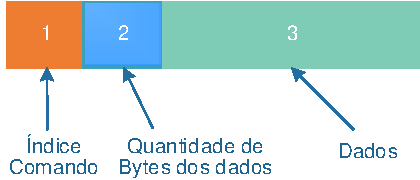
\includegraphics[width=10cm]{img8}  %pode alterar o tamanho
					\caption[Estrutura de um pacote I2C]{\label{img8}Estrutura de um pacote I2C}
				\end{center}		
			\end{figure}
			
			Como dito anteriormente, os dados que representam o estado do sistema, não correspondem a um array de bytes. Portanto, foi necessário converter as informações float e digitais para bytes para possibilitar a transmissão do mesmo. No Arduino isso foi feito utilizando a declaração union. Essa técnica permite variáveis de diferentes tipos ocupem uma mesma região de memória, o que possibilita que a estrutura de dados anteriormente criada possua a sua representação em um array de bytes, o que é necessário para transmissão via I2C. O \autoref{cod:dadosi2c} corresponde a implementação feita.
			
			Para correta interpretação dos comandos enviados pelo mestre, foi necessário mapear ações de acordo com o índice de comando criado, ou seja, definir um protocolo básico de comunicação.
			A relação entre o índice de comando e a ação correspondente é mostrada na \autoref{tbl5}. A interpretação e execução dos comandos é feita na função onReceive. Se o comando é uma solicitação de dados, o envio é realizado na função onRequest.
						
			\begin{listing}
				\begin{minted}[bgcolor=bg,breaklines=true,tabsize=2, baselinestretch=1,fontsize=\footnotesize]{cpp}
				//estrutura de dados para envio i2c
				typedef struct processData{
					float temp1;
					float temp2;
					float temp3;
					float temp4;
					float hotflow;
					float coldflow;
					float pump_speed;
					byte bstatus;
					byte chksum;
				};
				
				typedef union I2C_Send{ //compartilha a mesma área de memória
					processData data;
					byte I2C_packet[sizeof(processData)];
				};				
				\end{minted}
				\caption{Estrutura de dados do sistema}
				\label{cod:dadosi2c}
			\end{listing}
		
		\begin{table}[!htb]
			\centering
			\caption{Definição das interpretações de comando}
			\label{tbl5}
			\def\arraystretch{1.3}
			\begin{tabular}{c p{11cm}}
				\hline
				\multicolumn{1}{c}{\textbf{Índice Comando}} & \multicolumn{1}{c}{\textbf{Ação}} \\ \hline
				
				6 & Enviar dados do sistema para o mestre \\
				49 & Ligar a bomba \\ %\hline
				50 & Desligar a bomba \\ %\hline  
				51 & Ligar aquecedor \\ %\hline
				52 & Desligar o aquecedor \\ %\hline
				53 & Alterar velocidade da bomba \\ %\hline
				\hline
			\end{tabular}
		\end{table}
		
	\section{Preparação do Raspberry PI}
		\subsection{Instalação do sistema operacional}
			Conforme mencionado na \textcolor{red}{seçãoX}, o Raspberry não possui um HD interno. Portanto, é necessário instalar o sistema operacional em um microUSB, que faz o papel de HD. O Rpi suporta vários sistemas operacionais, sendo que o sistema operacional padrão é o Raspian, uma adaptação de uma distribuição Debian\footnote{\url{https://www.debian.org/intro/about}}. Foi utilizada a versão ``Raspian Stretch With Desktop'', disponível no link \url{https://www.raspberrypi.org/downloads/raspbian/}. Basicamente, deve-se extrair a imagem baixada para o microUSB. Após esse procedimento o Raspberry Pi já pode ser inicializado.
		
		\subsection{Ativação do protocolo I2C}
			O I2C não vem habilitado por padrão no sistema operacional. É necessário entrar nas configurações do Rpi e habilitá-lo. Os passos para realizar esse procedimento estão descritos por \textcite{matt2014}. Para verificar se o i2c está corretamente habilitado, deve-se abrir um terminal e digitar o comando ``sudo i2cdetect -y 1''. O resultado é exibido na \autoref{img9}.
			
			\begin{figure}[!htb]	
				%\centering
				\captionsetup{justification=centering}
				\begin{center}
					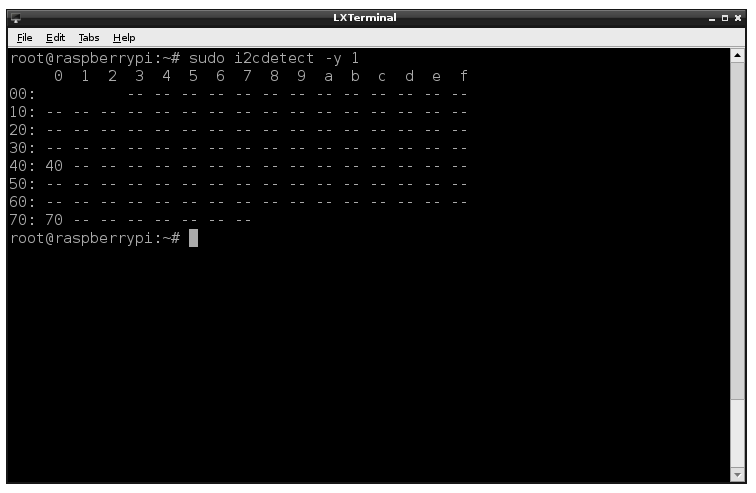
\includegraphics[width=10cm]{img9}  %pode alterar o tamanho
					\caption[I2C habilitado]{\label{img9}I2C habilitado}
				\end{center}		
			\end{figure}
		
		\subsection{Instalação de Pacotes - Python}
			O sistema operacional Raspian já possui duas versões instaladas de Python: 2.7 e 3.4. A primeira, mesmo sendo mais antiga ainda é muito utilizada pela comunidade devido à grande quantidade de pacotes desenvolvidos para essa versão; a segunda, é uma das versões mais novas disponíveis para Python.
			
			Os códigos do Gateway e do WebServer foram desenvolvidos com a versão 3.4. Antes do começo do desenvolvimento é necessário instalar os pacotes necessários para executar o projeto. Os pacotes a serem instalados dependem do propósito e característica do sistema a ser desenvolvido. É muito comum desenvolvedores trabalharem em diferentes projetos, portanto a tarefa de gerenciar os pacotes para cada projeto torna-se trabalhosa. Para isso, o Python disponibiliza a instalação de ambientes virtuais na máquina. Ambientes virtuais são diretórios para armazenar os pacotes necessários para determinados projetos. Assim, é possível isolar os arquivos de cada desenvolvimento, facilitando a mudança de um projeto para o outro \cite{kyle2017}. A utilização de ambientes virutais em Python é uma boa prática de programação e foi utilizada.
			
			Para instalar um ambiente virtual na versão python 3, é necessário utilizar os comandos descritos no \autoref{cod:venv}. Uma vez instalado, é necessário ativar o ambiente virtual. O  \autoref{cod:activate_venv} contém o código para ativá-lo. Após ativado, devem-se instalar os pacotes necessários para o projeto.  Os pacotes e as versões instaladas estão listados na \autoref{tbl6}
			
			\begin{listing}
				\begin{minted}[bgcolor=bg,breaklines=true,tabsize=2, baselinestretch=1,fontsize=\footnotesize]{bash}
				#navegar até a pasta onde se deseja instalar o ambiente virtual
				pi@raspberry $ cd pfc_env
				
				#instalar pacote virtual env
				pi@raspberry $ pip install virtualenv
				
				#criar um ambiente virtual chamado env
				pi@raspberry $ virtual env			
				\end{minted}
				\caption{Comandos para criação de um ambiente virtual}
			\label{cod:venv}
			\end{listing}
		
			\begin{listing}
				\begin{minted}[bgcolor=bg,breaklines=true,tabsize=2, baselinestretch=1,fontsize=\footnotesize]{bash}
				#ativar o diretório virtual
				pi@raspberry $ source pfc_env/bin/activate
				
				#caso o nome do diretório apareça entre parenteses como abaixo, o diretório foi ativado com sucesso
				(env) pi@raspberry $ 		
				\end{minted}
				\caption{Comandos para criação de um ambiente virtual}
				\label{cod:activate_venv}
			\end{listing}

			
			\begin{table}[!htb]
				\centering
				\caption{Pacotes necessários para o projeto}
				\label{tbl6}
				\def\arraystretch{1.3}
				\begin{tabular}{c c}
					\hline
					\multicolumn{1}{c}{\textbf{Pacote}} & \multicolumn{1}{c}{\textbf{Versão}} \\ \hline
					
					Smbus & v1.9.2 \\
					Django & v1.9.2 \\ %\hline
					Pillow & v1.9.2 \\ %\hline  
					\hline
				\end{tabular}
			\end{table}
		
			\begin{listing}
				\begin{minted}[bgcolor=bg,breaklines=true,tabsize=2, baselinestretch=1,fontsize=\footnotesize]{bash}
				#ativar o diretório virtual
				#o comando é pip install NomePacote== Versão. Exemplo:
				(env) pi@raspberry $ pip install Django==1.9.6					
				\end{minted}
				\caption{Comando para a instalação de pacotes Python}
				\label{cod:install}
			\end{listing}
		
			Todos os pacotes, com exceção do Smbus, podem ser instalados através do comando exibido no \autoref{cod:install}. É necessário ativar o ambiente virtual antes de efetuar os comandos. Para a instalação do Smbus, é necessário seguir os passos descritos por \textcite{dipto2015}. 
			
		
		
		\section{Código do Gateway}
			O código fonte completo do gateway está disponibilizado no Github, no link: \url{https://github.com/felipefonsecabh/PFC/blob/PyServeri2c/arduinoserver.py}
			
			
			
			
			